% MA4128

% https://www3.nd.edu/~rwilliam/stats1/OLS-SPSS.pdf
%http://psychweb.psy.umt.edu/denis/datadecision/front/stat_II_2011/psyx_521_multiple_regression_part_II.pdf

% ftp://public.dhe.ibm.com/software/analytics/spss/documentation/statistics/20.0/en/client/Manuals/IBM_SPSS_Regression.pdf

%http://www.education.umd.edu/EDMS/fac/Harring/Past-Classes/EDMS651/Notes/LRA-3.pdf

% http://www.psych.yorku.ca/lab/psy6140/lectures/ModelSelection2x2.pdf

%http://philosophy.wisc.edu/forster/220/simplicity.html

%http://statistics.uchicago.edu/~s220e/Lect/lec21.pdf

%http://publib.boulder.ibm.com/infocenter/spssstat/v20r0m0/index.jsp?topic=%2Fcom.ibm.spss.statistics.help%2Fsyn_regression_criteria_variable_selection.htm

\documentclass[a4paper,12pt]{article}
%%%%%%%%%%%%%%%%%%%%%%%%%%%%%%%%%%%%%%%%%%%%%%%%%%%%%%%%%%%%%%%%%%%%%%%%%%%%%%%%%%%%%%%%%%%%%%%%%%%%%%%%%%%%%%%%%%%%%%%%%%%%%%%%%%%%%%%%%%%%%%%%%%%%%%%%%%%%%%%%%%%%%%%%%%%%%%%%%%%%%%%%%%%%%%%%%%%%%%%%%%%%%%%%%%%%%%%%%%%%%%%%%%%%%%%%%%%%%%%%%%%%%%%%%%%%
\usepackage{eurosym}
\usepackage{vmargin}
\usepackage{amsmath}
\usepackage{graphics}
\usepackage{epsfig}
\usepackage{framed}
\usepackage{subfigure}
\usepackage{fancyhdr}

\setcounter{MaxMatrixCols}{10}
%TCIDATA{OutputFilter=LATEX.DLL}
%TCIDATA{Version=5.00.0.2570}
%TCIDATA{<META NAME="SaveForMode"CONTENT="1">}
%TCIDATA{LastRevised=Wednesday, February 23, 201113:24:34}
%TCIDATA{<META NAME="GraphicsSave" CONTENT="32">}
%TCIDATA{Language=American English}

\pagestyle{fancy}
\setmarginsrb{20mm}{0mm}{20mm}{25mm}{12mm}{11mm}{0mm}{11mm}
\lhead{MA4128} \rhead{Kevin O'Brien} \chead{Week 8} %\input{tcilatex}

%http://www.electronics.dit.ie/staff/ysemenova/Opto2/CO_IntroLab.pdf
\begin{document}

\tableofcontents
\newpage
\section{SLR Example}


The data give the yields of cotton and irrigation levels in the Salt River Valley for different plots of land. Each plot was on Maricopa sandy loam soil. The variables are as follows:
\begin{itemize}
\item \textbf{Irrigation} The amount of irrigation water applied in feet per acre. This is the predictor variable.
\item \textbf{Yield} The yield of Pima cotton in pounds per acre. This is the response variable.
\end{itemize}
\begin{center}
\begin{tabular}{|c|c|c||c|c|c|}
  \hline
  % after \\: \hline or \cline{col1-col2} \cline{col3-col4} ...
  Observation & Irrigation & Yield & Observation & Irrigation & Yield \\\hline
  1 & 1.8	& 260 & 8  &  1.5	& 280 \\
  2 & 1.9	& 370 & 9  & 1.5	& 230 \\
  3 & 2.5	& 450 & 10 & 1.2	& 180 \\
  4 & 1.4	& 160 & 11 & 1.3	& 220 \\
  5 & 1.3	& 90  & 12 & 1.8	& 180 \\
  6 & 2.1	& 440 & 13 & 3.5	& 400 \\
  7 & 2.3	& 380 & 14 & 3.5	& 650 \\
  \hline
\end{tabular}
\end{center}


%\begin{figure}[h!]
%\begin{center}
%  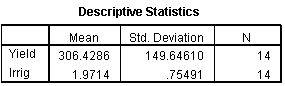
\includegraphics[scale=0.8]{SLR1.png}
%  \caption{SPSS output.}\label{SLR1}
%\end{center}
%\end{figure}


\begin{center}
\begin{table}[htbp]
  \centering
  \caption{Add caption}
    \begin{tabular}{|rrrr|}
    %\toprule
    \hline
    \multicolumn{4}{c}{Descriptive Statistics}  \\
    \hline % midrule
          & \multicolumn{1}{|c|}{Mean} & \multicolumn{1}{|c|}{Std. Deviation} & \multicolumn{1}{|c|}{N} \\
    \multicolumn{1}{|l|}{Yield} & 306.4286 & 149.6461 & 14 \\
    \multicolumn{1}{|l|}{Irrig} & 1.971429 & 0.754911 & 14 \\
    %\bottomrule
    \hline
    \end{tabular}%

\end{table}%
\end{center}

Next we are given the output from the correlation analysis and the regression ANOVA.

%\begin{figure}[h!]
%\begin{center}
%  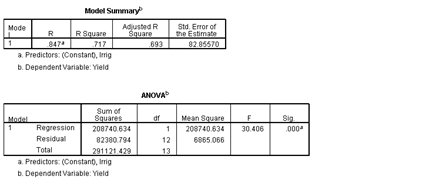
\includegraphics[width=160mm]{SLR3.jpg}
%  \caption{SPSS output.}\label{SLR1}
%\end{center}
%\end{figure}

The intercept and slope estimate are determined by examining the ``coefficients".
%\begin{figure}[h!]
%\begin{center}
%  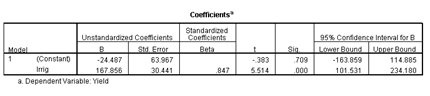
\includegraphics[width=150mm]{SLR2.jpg}
%  \caption{SPSS output.}\label{SLR1}
%\end{center}
%\end{figure}












%-----------------------------------------------------------------------------------------%
\section{Correlation}

Pearson's correlation coefficient ($r$) is a measure of the strength of the 'linear' relationship between two quantitative variables. A major assumption is the normal distribution of variables. If this assumption is invalid (for example, due to outliers), the non-parametric equivalent Spearman's rank correlation should be used.

\subsection{Formal test of Correlation}
\subsection{Lurking variables and Spurious Correlation}
Spurious Correlations. Although you cannot prove causal relations based on correlation coefficients, you can still identify so-called spurious correlations; that is, correlations that are due mostly to the influences of "other" variables. For example, there is a correlation between the total amount of losses in a fire and the number of firemen that were putting out the fire; however, what this correlation does not indicate is that if you call fewer firemen then you would lower the losses. There is a third variable (the initial size of the fire) that influences both the amount of losses and the number of firemen. If you "control" for this variable (e.g., consider only fires of a fixed size), then the correlation will either disappear or perhaps even change its sign. The main problem with spurious correlations is that we typically do not know what the "hidden" agent is. However, in cases when we know where to look, we can use partial correlations that control for (partial out) the influence of specified variables.



\subsection{Simpson's Paradox}
\subsection{Rank correlation}
Spearman's Rank correlation coefficient


\subsection{Partial Correlation}
Partial correlation analysis involves studying the linear relationship between two variables after excluding the effect of one or more independent factors.

%-----------------------------------------------------------------------------------------%
\section{Multiple Linear Regression}
Multiple regression: To quantify the relationship between several independent (predictor) variables and a dependent (response) variable. The coefficients ($a, b_{1} to b_{i}$) are estimated by the least squares method, which is equivalent to maximum likelihood estimation. A multiple regression model is built upon three major assumptions:

\begin{enumerate}
\item The response variable is normally distributed,
\item The residual variance does not vary for small and large fitted values (constant variance),
\item The observations (explanatory variables) are independent.
\end{enumerate}


\subsection{Dummy Variables}
A dummy variable is a numerical variable used in regression analysis to represent subgroups of the sample in your study. In research design, a dummy variable is often used to distinguish different treatment groups. In the simplest case, we would use a 0,1 dummy variable where a person is given a value of 0 if they are in the control group or a 1 if they are in the treated group. Dummy variables are useful because they enable us to use a single regression equation to represent multiple groups. This means that we don't need to write out separate equation models for each subgroup.

\subsection{Estimates}

%-----------------------------------------------------------------------------------------%

\newpage



\section{Information Criterions}


We define two types of information criterion: the Bayesian Information
Criterion (BIC) and the Akaike Information Criterion (AIC). In AIC and BIC, we choose the model that
has the minimum value of:
\[AIC = −2log(L)+2m,\]
\[BIC = −2log(L)+mlogn\]

where
\begin{itemize}
\item L is the likelihood of the data with a certain model,
\item n is the number of observations and
\item m is the number of parameters in the model.
\end{itemize}
\subsection{AIC}
The Akaike information criterion is a measure of the relative \textbf{goodness of fit} of a statistical model.

When using the AIC for selecting the parametric model class, choose
the model for which the AIC value is lowest.

\end{document} 




\section{Training and validation}
%http://www.jmp.com/support/help/Validation_2.shtml
Using Validation and Test Data

%When you have sufficient data, you can subdivide your data into three parts called the training, validation, and test data. During the selection process, models are fit on the training data, and the prediction error for the models so obtained is found by using the validation data. This prediction error on the validation data can be used to decide when to terminate the selection process or to decide what effects to include as the selection process proceeds. Finally, once a selected model has been obtained, the test set can be used to assess how the selected model generalizes on data that played no role in selecting the model.

In some cases you might want to use only training and test data. For example, you might decide to use an information criterion to decide what effects to include and when to terminate the selection process. In this case no validation data are required, but test data can still be useful in assessing the predictive performance of the selected model. In other cases you might decide to use validation data during the selection process but forgo assessing the selected model on test data. 
%Hastie, Tibshirani, and Friedman (2001) note that it is difficult to give a general rule on how many observations you should assign to each role. They note that a typical split might be 50\% for training and 25% each for validation and testing.




\section{Multiple Linear Regression}
\subsection{What is Multiple Linear Regression}

Multiple regression is a statistical technique that allows us to predict a numeric value on the response variable on the basis of the observed values on several other independent variables.

Suppose we were interested in predicting how much an individual enjoys their job. Variables such as salary, extent of academic qualifications, age, sex, number of years in full-time employment and socioeconomic status might all contribute towards job satisfaction. If we collected data on all of these variables, perhaps by surveying a few hundred members of the public, we would be able to see how many and which of these variables gave rise to the most accurate prediction of job satisfaction. We might find that job satisfaction is most accurately predicted by type of occupation, salary and years in full-time employment, with the other variables not helping us to predict job satisfaction.

\[\hat{y} = b_0 + b_1x_1 + b_2x_2 + \ldots \]

\begin{itemize}
	\item $\hat{y}$ is the \textbf{\textit{fitted value}} for the dependent variable \textbf{$Y$}, given a linear combination of values for the independent valriables.
	
	\item $x_1$ is the value for independent variable \textbf{$X_1$}.
	\item $b_o$ is the constant regression estimate ( commonly known as the \textbf{Intercept Estimate} in the case of simple linear regression).
\end{itemize}
\newpage
\section{Terminology}
\subsection{Beta (standardised regression coefficients)}
The beta value is a measure of how strongly each predictor variable influences the
response variable. The beta is measured in units of standard deviation. For example,
a beta value of 2.5 indicates that a change of one standard deviation in the predictor
variable will result in a change of 2.5 standard deviations in the response variable.
Thus, the higher the beta value the greater the impact of the predictor variable on
the response variable.


The Standardized Beta
Coefficients give a measure of the
contribution of each variable to
the model. A large value indicates
that a unit change in this
predictor variable has a large
effect on the criterion variable.
The t and Sig (p) values give a
rough indication of the impact of
each predictor variable – a big
absolute t value and small p value
suggests that a predictor variable
is having a large impact on the
criterion variable.

%\subsection{R, R Square, Adjusted R Square}
%
%R is a measure of the correlation between the observed value and the predicted value of the criterion variable. In our example this would be the correlation between the levels of job satisfaction reported by our participants and the levels predicted for
%them by our predictor variables.
%
%R Square (R2) is the square of this measure of
%correlation and indicates the proportion of the variance in the criterion variable which is accounted for by our model – in our example the proportion of the
%variance in the job satisfaction scores accounted for by our set of predictor variables
%(salary, etc.).
%
%In essence, this is a measure of how good a prediction of the criterion variable we can make by knowing the predictor variables.
% However, R square tends to somewhat over-estimate the success of the model when applied to the real world, so an Adjusted R Square value is calculated which takes into account the number of variables in the model and the number of observations (participants) our model is based on. This Adjusted R Square value gives the most useful measure of the success of our model. If, for example we have an Adjusted R Square value of 0.75 we can say that our model has accounted for 75\% of the variance in the criterion
%variable.
%
%Adjusted $R^2$ is used to compensate for the addition of variables to the model.  As more independent variables are added to the regression model, unadjusted R2 will generally increase but there will never be a decrease.  This will occur even when the additional variables do little to help explain the dependent variable.  To compensate for this, adjusted R2 is corrected for the number of independent variables in the model.  The result is an adjusted R2 than can go up or down depending on whether the addition of another variable adds or does not add to the explanatory power of the model.  Adjusted R2 will always be lower than unadjusted.
%
%It has become standard practice to report the adjusted R2, especially when there are multiple models presented with varying numbers of independent variables.



%-------------------------------------------------------------- %
\newpage
\section{ANOVA}
In ANOVA we are trying to determine how much of the variance is
accounted for by our manipulation of the independent variables (relative to the percentage of the variance we cannot account for).
%------------------------------------------------------------- %
\newpage

%
%\subsection{Checking prediction success: using training and validation sets}
%Another approach is to randomly assign your cases to two datasets. The first, called
%the training set, is used to calculate the regression.
%
%The second is called the validation set. The predicted score is calculated for all the cases in the validation set, but as we
%already have their actual scores, we can find the residuals and their standard
%deviation.

%%--------------------------------------------------------------------------- %
%\newpage
%
%
%
%%------------------------------------------------------------%
%\subsection{Adjusted R square}
%
%In a multiple linear regression model, adjusted R square measures the proportion of the variation in the dependent variable
%accounted for by the independent variables.


%------------------------------------------------------------%

%\subsection{Model Selection}
%
%Model selection is the task of selecting a statistical model from a set of potential models, given data.


%------------------------------------------------------------%


\end{document}